% Modified Template by Kevin Multani, original by: Jonathan Ward

\documentclass[12pt]{article} 
\usepackage[english]{babel}
\usepackage[utf8]{inputenc}
\usepackage{amsmath} % AMS Math Package
\usepackage{amsthm} % Theorem Formatting
\usepackage{amssymb} % Math symbols such as \mathbb
\usepackage{graphicx} % Allows for eps images
\usepackage{multicol} % Allows for multiple columns
\usepackage[dvips,letterpaper,margin=1in,bottom=1in]{geometry}
\usepackage{hyperref}
\usepackage{mathrsfs}
\usepackage{amsmath,amscd}
\usepackage[all,cmtip]{xy}
\usepackage{bbm}
\usepackage{titling}
\usepackage{fancyhdr}
\usepackage[]{physics}
\usepackage[makeroom]{cancel}
\usepackage{pdfpages}
\usepackage[]{mcode}

% ***********************************************************
% ********************** BEGIN TITLE PAGE *******************
% ***********************************************************
\newcommand*{\titleGM}{\begingroup % Create the command for including the title page in the document
\hbox{ % Horizontal box
\hspace*{0.2\textwidth} % Whitespace to the left of the title page
\rule{1pt}{\textheight} % Vertical line
\hspace*{0.05\textwidth} % Whitespace between the vertical line and title page text
\parbox[b]{0.75\textwidth}{ % Paragraph box which restricts text to less than the width of the page

{\noindent\Huge\bfseries The Story of the Deuteron}\\[2\baselineskip] % Title
{\large \textit{PHYS 473: Assignment 1}}\\[4\baselineskip]
{\large \textsc{ Kevin Multani }} % Author name

\vspace{0.5\textheight} % Whitespace between the title block and the publisher
{\noindent \today }\\[\baselineskip]
{\noindent Student Number: 33542127 }\\[\baselineskip] 
{\noindent \footnotesize All problems below are \textit{Copyright \copyright \space 2018 Javed Iqbal. All Rights Reserved.} }\\[\baselineskip]
	}
}
\endgroup}

 % Sets margins and page size
\pagestyle{fancy} 

\lhead{Kevin Multani}
\rhead{\today}
\rfoot{Page \thepage}
\cfoot{}

\makeatletter % Need for anything that contains an @ command 
\renewcommand{\maketitle} % Redefine maketitle to conserve space
{ \begingroup \vskip 10pt \begin{center} \Huge {\bf \@title}
	\vskip 10pt \large \@author \hskip 20pt \@date \end{center}
  \vskip 10pt \endgroup \setcounter{footnote}{0} }
\makeatother % End of region containing @ commands

% ***********************************************************
% ********************** END TITLE PAGE *********************
% ***********************************************************

% ***********************************************************
% ********************** BEGIN NEW COMMANDS *****************
% ***********************************************************

\renewcommand{\labelenumi}{(\alph{enumi})} % Use letters for enumerate
\let\vaccent=\v % rename builtin command \v{} to \vaccent{}

%% MISC
\newcommand{\ab}[1]{\left| #1 \right|} % for absolute value
\newcommand{\avg}[1]{\left< #1 \right>} % for average
\let\underdot=\d % rename builtin command \d{} to \underdot{}
\let\baraccent=\= % rename builtin command \= to \baraccent
\renewcommand{\=}[1]{\stackrel{#1}{=}} % for putting numbers above =
\providecommand{\fr}{\frac}
\providecommand{\RR}{\mathbb{R}}
\providecommand{\CC}{\mathbb{C}}
\providecommand{\NN}{\mathbb{N}}
\providecommand{\e}{\epsilon}
\DeclareMathOperator{\di}{d\!}
\newcommand*\ieval[3]{\left.#1\right\rvert_{#2}^{#3}}


%% Vectors
\renewcommand{\v}[1]{\ensuremath{\mathbf{#1}}} 
\newcommand{\gv}[1]{\ensuremath{\mbox{\boldmath$ #1 $}}} % for vectors of Greek letters
\newcommand{\uv}[1]{\ensuremath{\mathbf{\hat{#1}}}} % for unit vector
\providecommand{\wave}[1]{\v{\tilde{#1}}}

%% DERIVATIVES
\renewcommand{\d}[2]{\frac{d #1}{d #2}} % for derivatives
\newcommand{\dubd}[2]{\frac{d^2 #1}{d #2^2}} % for double derivatives
\newcommand{\pd}[2]{\frac{\partial #1}{\partial #2}} % for partial derivatives
\newcommand{\pdd}[2]{\frac{\partial^2 #1}{\partial #2^2}} % for double partial derivatives


% ***********************************************************
% ********************** END NEW COMMANDS *******************
% ***********************************************************

% ***********************************************************
% ********************** BEGIN NEW ENVS *********************
% ***********************************************************

% Theorem
\newenvironment{theorem}[2][Theorem]{\begin{trivlist}
\item[\hskip \labelsep {\bfseries #1}\hskip \labelsep {\bfseries #2.}]}{\end{trivlist}}
% Lemma
\newenvironment{lemma}[2][Lemma]{\begin{trivlist}
\item[\hskip \labelsep {\bfseries #1}\hskip \labelsep {\bfseries #2.}]}{\end{trivlist}}
% Corollary
\newenvironment{corollary}[2][Corollary]{\begin{trivlist}
\item[\hskip \labelsep {\bfseries #1}\hskip \labelsep {\bfseries #2.}]}{\end{trivlist}}

% Exercise
\newenvironment{exercise}[2][Exercise]{\begin{trivlist}
\item[\hskip \labelsep {\bfseries #1}\hskip \labelsep {\bfseries #2.}]}{\end{trivlist}}
% Problem
\newenvironment{problem}[2][Problem]{\begin{trivlist}
\item[\hskip \labelsep {\bfseries #1}\hskip \labelsep {\bfseries #2.}]}{\end{trivlist}}
% Question
\newenvironment{question}[2][Question]{\begin{trivlist}
\item[\hskip \labelsep {\bfseries #1}\hskip \labelsep {\bfseries #2.}]}{\end{trivlist}}
% Solution
\newenvironment{solution}{\begin{proof}[Solution]}{\end{proof}}

% ***********************************************************
% ********************** END NEW ENVS ***********************
% ***********************************************************

% ***********************************************************
% ********************** END TITLEPAGE **********************
% ***********************************************************


\begin{document}

    \begin{titlingpage}
		\titleGM
	\end{titlingpage}
	\clearpage
	\setcounter{page}{1}

%%%%%%%%%%%%%% PROBLEM 1

	\begin{problem}{1} 
        Consider the deuteron wave function for a finite square-well potential, 
        
        $$
        u(r)=
        \begin{cases}
            A\sin(kr) & r < R\\
            Ce^{\gamma r} & r > R\\
        \end{cases}
        $$
        where,
        \begin{align*}
            k &= \sqrt{\frac{2\mu}{\hbar^2}\left(V_0 - B\right)} & \gamma = \sqrt{\frac{2\mu}{\hbar^2}B}\\ & & \\
            \mu &= 469.46 \text{ MeV}/c^2 & B = 2.2 \text{ MeV}
        \end{align*}
	    Using the normalization condition,
	    
	    $$
	    \int_0^\infty \left(u(r)\right)^2 \di r = 1,
	    $$
	    show that the normalization constants $A$ and $C$ satisfy,
	    
	    $$
	    \frac{A^2}{2}\left(R - \frac{\cos(kR)\sin(kR)}{k}\right) + \frac{C^2}{2\gamma}e^{-2\gamma R} = 1.
	    $$
	    Now combining the above equation with the continuity of wave function and its derivative at $r = R$, 
	    
	    \begin{align*}
	        A\sin(kR) &= Ce^{-\gamma R}\\
	        Ak\cos(kR) &= -\gamma Ce^{-\gamma R},
	    \end{align*}
	    show that $A$ and $C$ are given by,
	    
	    \begin{align*}
	        A^2 &= \frac{2\gamma}{1 + \gamma R} & C^2 &= \frac{2\gamma}{1 + \gamma R} \sin^2(kR)e^{2\gamma R}. 
	    \end{align*}
	\end{problem}

    \begin{solution} 
    	To do the first part of the problem we follow the hint provided, beginning with the normalization condition of the deuteron wave function,
    	$$
    	\int_0^{\infty} \left(u(r)\right)^2 \di r = 1
    	$$
    	\begin{align*}
    	    \int_0^R A^2 \sin^2(kr) \di r + \int_R^\infty C^2 e^{-2\gamma r} \di r &= 1\\\\
    	    \frac{A^2}{2}\int_0^R \left( 1 - \cos(2kr) \right) \di r + \ieval{\frac{C^2}{-2\gamma} e^{-2\gamma r}}{R}{\infty} &= 1 \\\\
    	   \frac{A^2}{2} \left(R - \frac{\sin(2kR)}{2k}\right) + \frac{C^2}{2\gamma}e^{-2\gamma R} &= 1
    	\end{align*}
    	\begin{align}
    	    \frac{A^2}{2}\left(R - \frac{\cos(kR)\sin(kR)}{k}\right) + \frac{C^2}{2\gamma}e^{-2\gamma R} &= 1,
    	\end{align}
    	as required. In the above steps, there were two trigonometric identities used: $\sin^2(x) = \tfrac{1}{2}\left(1-\cos(2x)\right)$ and $\sin(2x) = 2\sin(x)\cos(x)$ to obtain $\text{(1)}$.\\
    	
    	\noindent For the next part, a bit more is needed. First we start off discovering some identities from the boundary conditions,
    	\begin{align*}
    	    A\sin(kR) &= Ce^{-\gamma R}\\
    	    kA\cos(kR) &= -\gamma Ce^{-\gamma R} \Rightarrow
    	\end{align*}
    	\begin{align}
    	    A^2 \sin^2(kR) &= C^2 e^{-2\gamma R}\\
    	    A^2 \cos^2(kR) &= \frac{\gamma^2}{k^2}C^2e^{-2\gamma R}
    	\end{align}
    	$$
    	\text{(2) + (3)} \Rightarrow
    	$$
    	\begin{align}
    	    C^2 &= \frac{e^{2\gamma R}}{\left(1 + \frac{\gamma^2}{k^2}\right)} A^2
    	\end{align}
    	Furthermore, we can divide the two equations given by the boundary conditions to obtain,
    	\begin{align}
    	    \frac{\cos(kR)}{\sin(kR)} &= -\frac{\gamma}{k} \Longleftrightarrow\\
    	    \frac{\cos^2(kR)}{\sin^2(kR)} &= \frac{\gamma^2}{k^2}
    	\end{align}
        Now we are ready to do some simplification, starting with equation $\text{(1)}$, we get,
        \begin{align*}
    	    \frac{A^2}{2}\left(R - \frac{\cos(kR)\sin(kR)}{k}\right) + \frac{C^2}{2\gamma}e^{-2\gamma R} &= 1 \\\\
    	    A^2\left(R\gamma - \frac{\gamma}{k}\cos(kR)\sin(kR)\right) + C^2e^{-2\gamma R} &= 2\gamma, \text{ plugging in (2) and (5)}\\\\
    	    A^2 \left( \gamma R + \frac{\cos(kR)}{\cancel{\sin(kR)}}\cos(kR)\cancel{\sin(kR)} + \sin^2(kR)\right) &= 2\gamma \\\\
    	    A^2 &= \frac{2\gamma}{1 + \gamma R}.
        \end{align*}
        To get $C^2$ we note, using $\text{(6)}$,
        \begin{align}
            \frac{1}{1 + \frac{\gamma^2}{k^2}} = \frac{\sin^2(kR)}{\sin^2(kR) + \cos^2(kR)} = \sin^2(kR) 
        \end{align}
        Plugging $\text{(7)}$ and $A^2$ into $\text{(4)}$, we get the desired result,
        \begin{align*}
            A^2 &= \frac{2\gamma}{1 + \gamma R} & C^2 &= \frac{2\gamma}{1 + \gamma R} \sin^2(kR)e^{2\gamma R}.
        \end{align*}
    \end{solution}
    \pagebreak

%%%%%%%%%%%%%% PROBLEM 2
    \begin{problem}{2}
        Using $R = 2.0 \text{ fm}$, $V_0 = 37 \text{ MeV}$ plot the deuteron wave function for $r = 0 \text{ fm}$ to $r = 15 \text{ fm}$.\\
        
        
    \end{problem}
    
    \begin{solution}
        Here is the plot of the wave function with the given parameters. The MATLAB code is attached at the end of the document. The dotted red line indicates where the discontinuity in the square-well potential is -- at $2 \text{ fm}$. For radial distances before $2 \text{ fm}$ the wave function is \textit{sine-like} and after $2 \text{ fm}$ the wave function is \textit{exponential-like}.
        
        \begin{figure}[h!]
            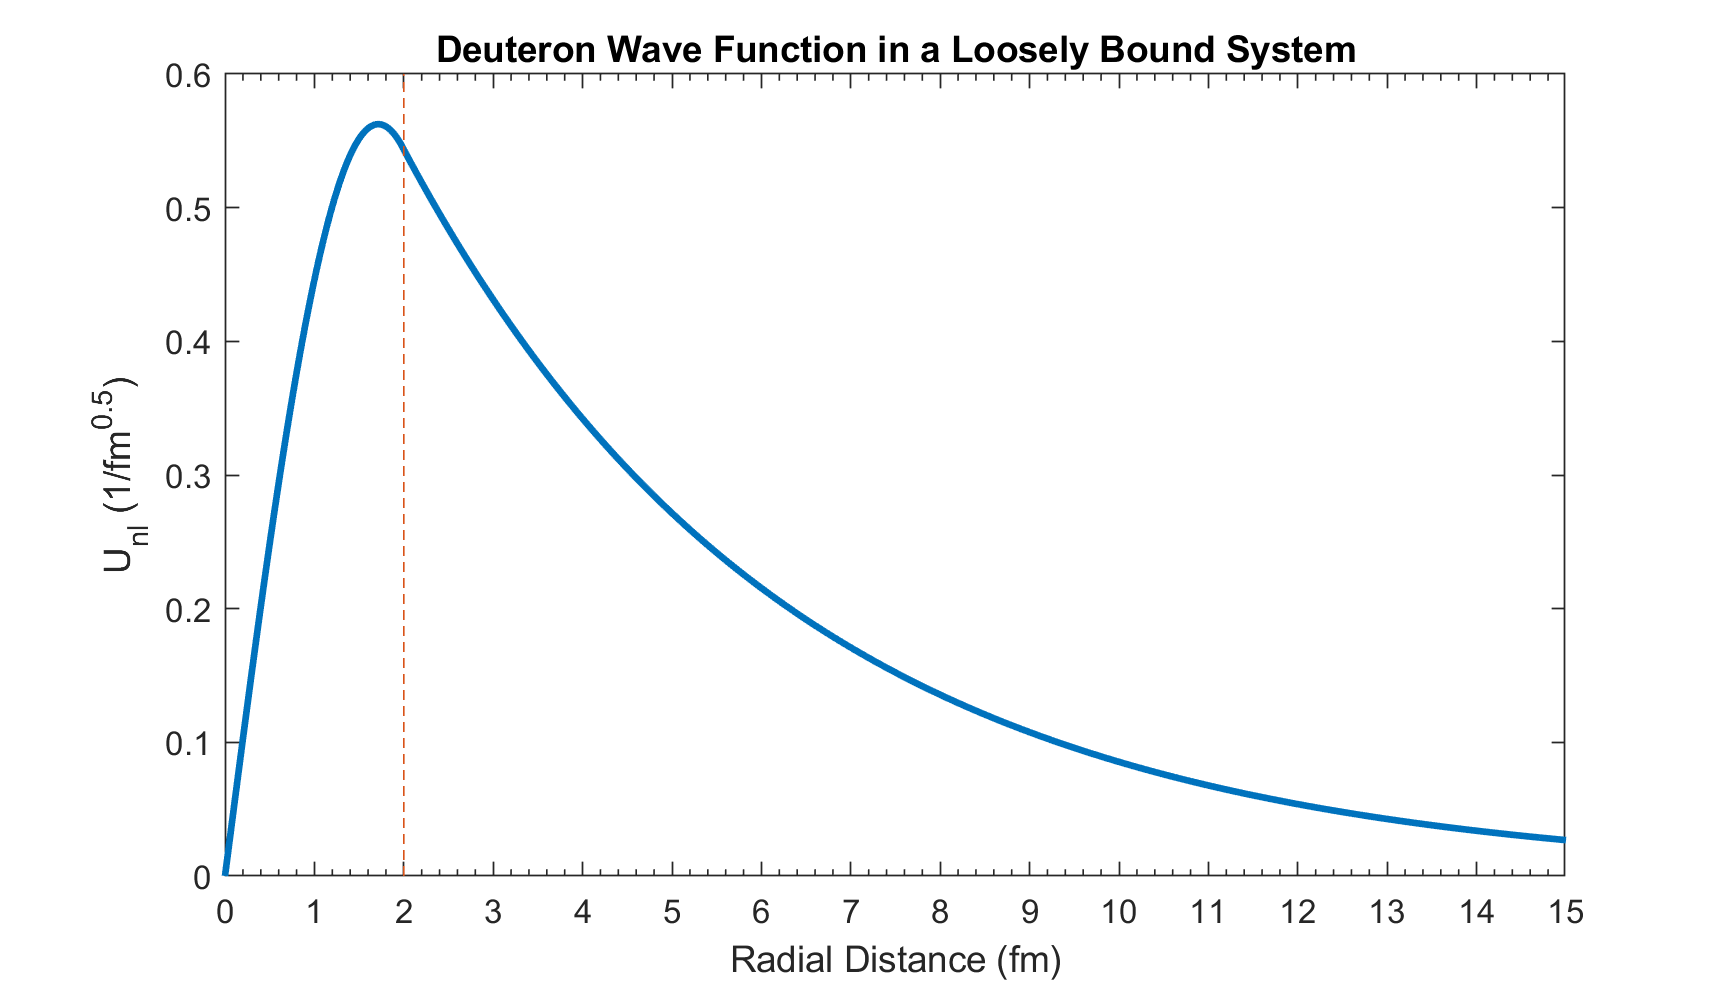
\includegraphics[scale=0.3]{fig1}
            \centering
        \end{figure}
        
        % \includepdf[scale=0.9, pages=-, pagecommand={}]{matlab_problems.pdf}
    \end{solution}
    
    \pagebreak

%%%%%%%%%%%%%% PROBLEM 3

    \begin{problem}{3}
        In the above equations $r$ is the relative separation between the proton and the neutron. The root-mean-square radius of the deuteron is given by,
        $$
        \avg{r_d^2} = \int_0^\infty \left(\frac{r}{2}\right)^2 \left(u(r)\right)^2 \di r
        $$
        Show (calculate numerically) that for the values of the constants used in problems $\text{(1)}$ and $\text{(2)}$ the rms radius $r_d$ is $1.92 \text{ fm}$. So the size of a deuteron (its diameter) is about $4 \text{ fm}$ implying that a deuteron is a rather loosely bound system.
    \end{problem}
    \begin{solution}
        Here are two outputs that verify the normalization condition of the wave function and the approximation for the rms radius. The code that generates the outputs is attached at the end of the document.
        \begin{figure}[h!]
            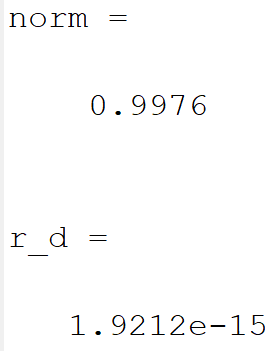
\includegraphics[scale=0.75]{output.PNG}
            \centering
        \end{figure}
        %
    \end{solution}
    
    \pagebreak
    
    \section*{MATLAB Code}
        \lstinputlisting{matlab_problems.m}
\end{document}